\subsubsection{Aktualisieren des Referenzscans (Janneke)}

Ein Problem mit unserer Implementation liegt darin, dass sich über die Zeit Fehler aufsummieren und die Scans immer weiter vom Original weg driften können. Ein möglicher Ansatz um dem entgegenzuwirken ist es den Referenzscan nicht in jedem Schritt, sondern nur ab und zu zu wechseln. Das heißt man arbeitet nicht jedes mal mit dem aktuellen und dem Scan aus dem vorherigen Schritt, sondern immer mit dem aktuellen und dem zuletzt festgelegten Referenzscan.

Also wird der Referenzscan, die ''Referenz-''Odometrie und sowohl der globale Rotationsoffset, als auch der globale Translationsoffset nur alle x-Schritte mit den aktuellen Werten überschrieben und nicht mehr am Ende jedes Schleifendurchgangs.

Dies bringt einen weiteren Update-Parameter der optimiert werden muss. Diese Optimierung erwies sich als relativ schwierig, da wir bereits einen COUNT-Parameter haben der bestimmt wie oft das Karten-Update überhaupt passiert.

\begin{figure}
	\centering
	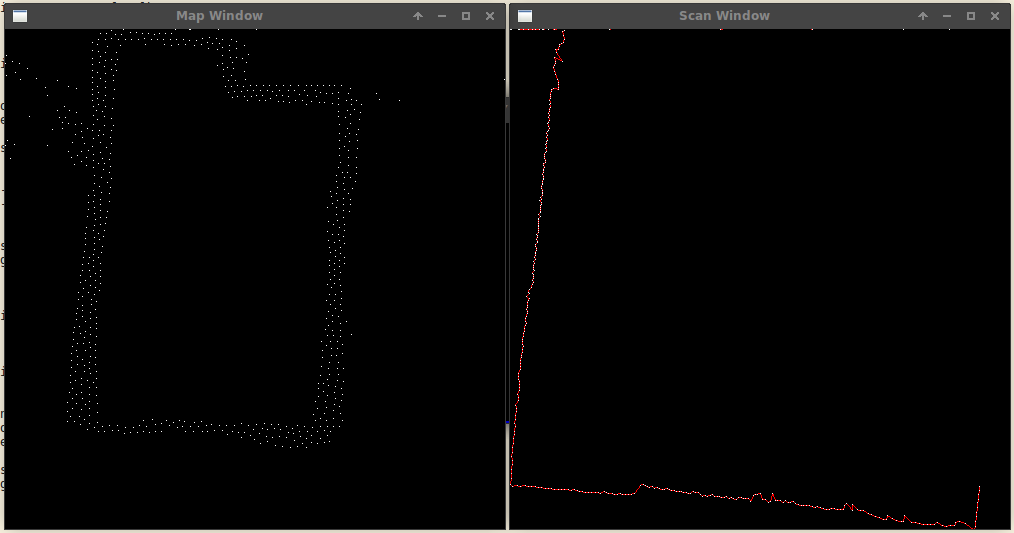
\includegraphics[width=14cm]{refTest_c1_r2_4min_2}
	\caption{Karten-Update jeden Schritt, Referenzscan-Update alle 2 Schritte, 4 Minuten Fahrzeit\newline}
	\label{fig:count1_r2_4min}
	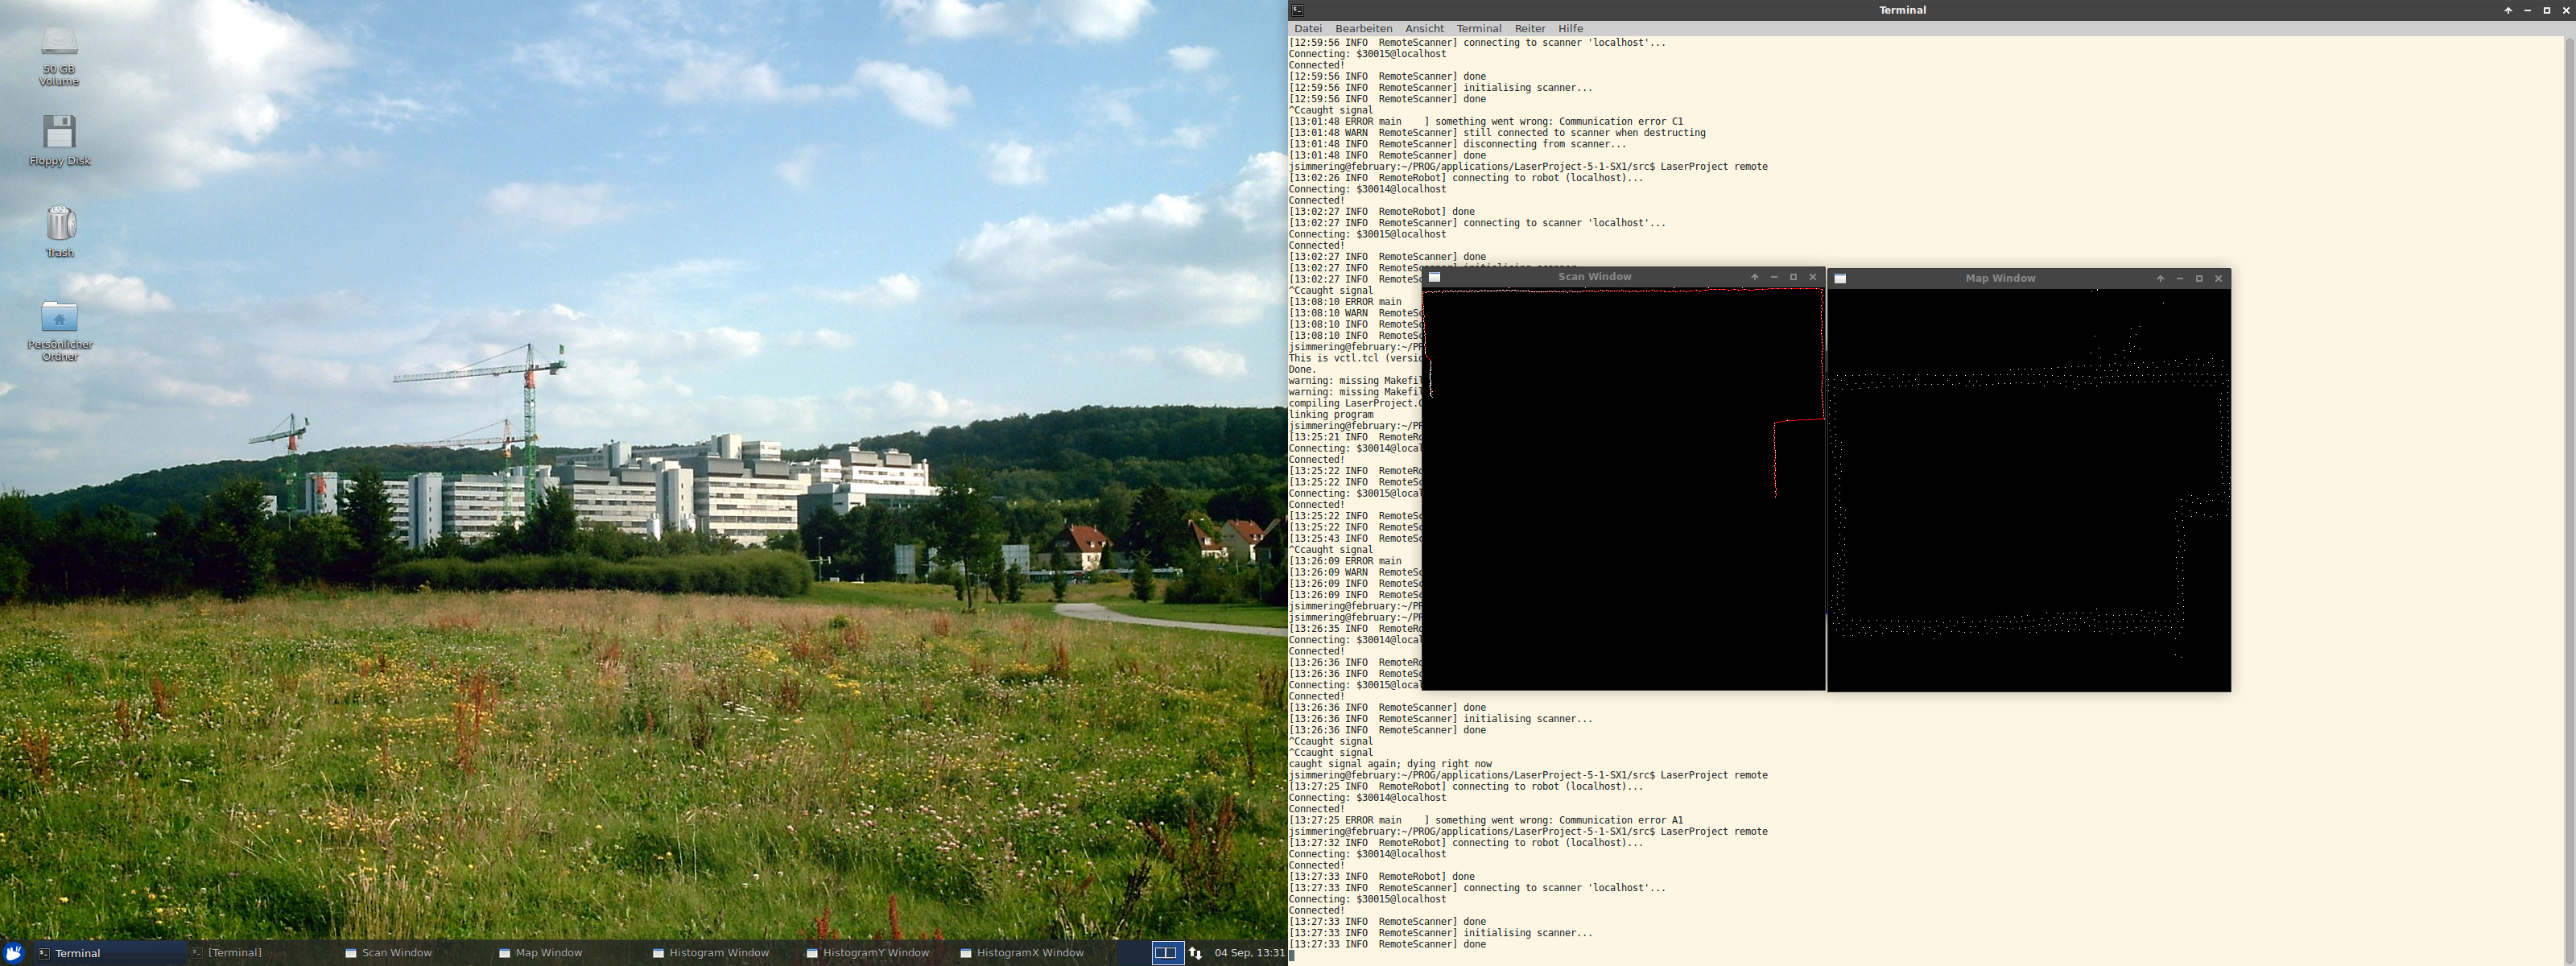
\includegraphics[width=14cm]{refTest_c4_r1_4min}
	\caption{Karten-Update alle 4 Schritte, Referenzscan-Update jeden Schritt, 4 Minuten Fahrzeit}
	\label{fig:count4_r1_4min}
\end{figure}

Bei der Optimierung des Update-Parameter haben wir verschiedene Count- und Update-Parameterkombinationen getestet. Dabei war auffällig, dass bei einem selteneren Referenzscan-Update das Verfahren schlechter funktioniert hat, wenn der Roboter engere Kurven gefahren ist, sich zum Beispiel in einer Sackgasse umgedreht hat. Dies ist dadurch zu erklären, dass der mehrere Scans alte Referenzscan und der aktuelle Scan wenig gleiche Teile des Raumes abdecken. Dadurch kann eine Korrelation der Beiden Scans nicht sinnvoll berechnet werden. Um dieses Problem ab zu mildern haben wir zunächst das Umdrehen des Roboters in einer Sackgasse blockierend um 180 Grad zu einem nicht blockierenden drehen auf der Stelle durch entgegengesetzte Radgeschwindigkeiten ersetzt. Außerdem haben wir insgesamt die Geschwindigkeit des Roboters reduziert, was sowohl der Version mit einem Referenzscan-Update in jedem Schritt als auch der mit weniger Updates geholfen hat.

Letztendlich ergaben unsere Test, dass unsere Implementation am besten funktioniert, wenn man entweder in jedem Schritt ein Karten-Update ausführt, aber den Referenzscan nur alle zwei Schritte updatet (siehe Abbildung~\ref{fig:count1_r2_4min}), oder nur jeden 4. Schritt ein Karten-Update ausführt, dafür aber in jedem dieser Schritte auch den Referenzscan wechselt (siehe Abbildung~\ref{fig:count4_r1_4min}). Da die zweite Version etwas besser zu funktionieren schien verwenden wir diese.